\newpage
\part{Appendix}
\appendix

\section{Test Evidence}
    
    A google drive folder where video evidence of the tests can be found here: \url{https://bit.ly/2WyO9L0}.

    \subsection{Predictions}
    The following graphs show real prices vs. the prediction made for that timestep for each network on a sample of the test data. Real prices are in blue, predictions in orange.

    \begin{figure}[htbp]
        \centering
        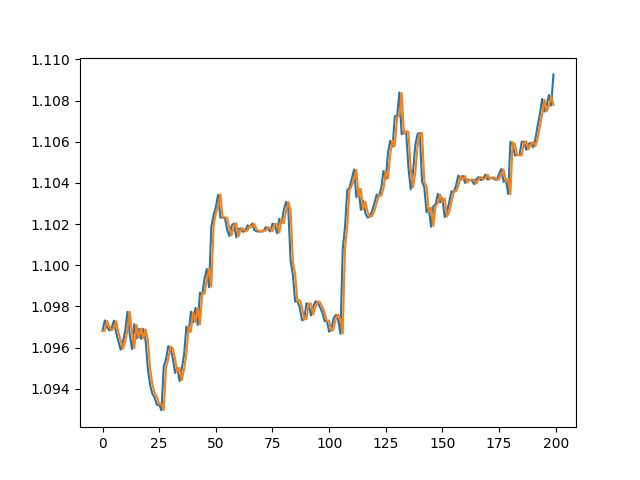
\includegraphics[width=0.9\textwidth]{15.png}
        \caption{15 minute predictions}
        \label{fig:15}
    \end{figure}

    \begin{figure}[htbp]
        \centering
        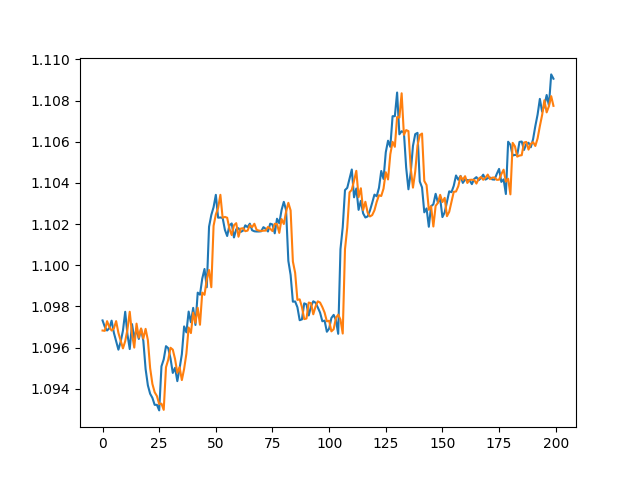
\includegraphics[width=0.9\textwidth]{30.png}
        \caption{30 minute predictions}
        \label{fig:30}
    \end{figure}

    \begin{figure}[htbp]
        \centering
        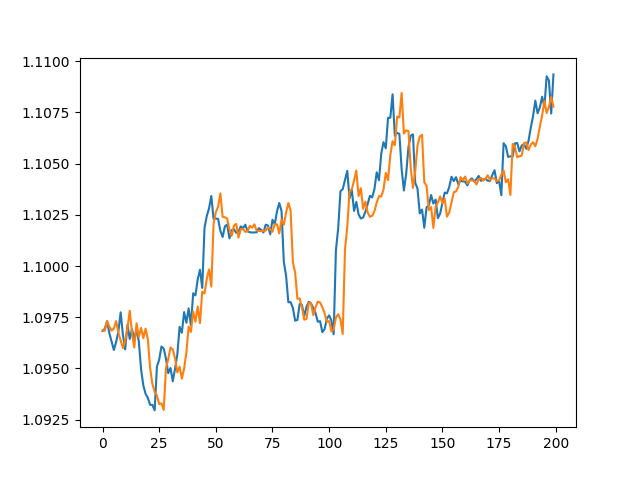
\includegraphics[width=0.9\textwidth]{60.png}
        \caption{1 hour predictions}
        \label{fig:60}
    \end{figure}

    \begin{figure}[htbp]
        \centering
        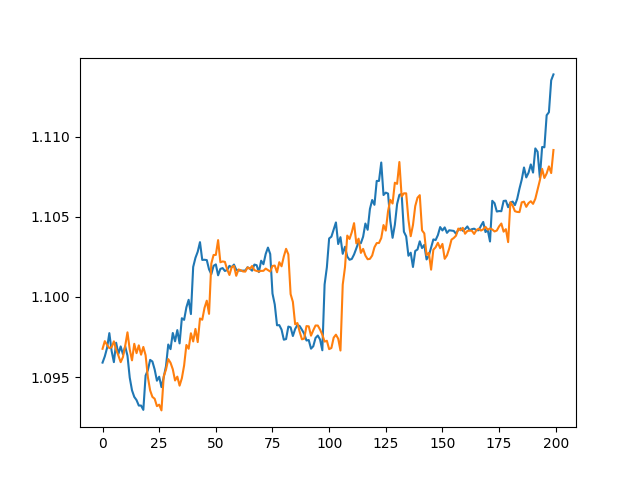
\includegraphics[width=0.9\textwidth]{120.png}
        \caption{2 hour predictions}
        \label{fig:120}
    \end{figure}

    \begin{figure}[htbp]
        \centering
        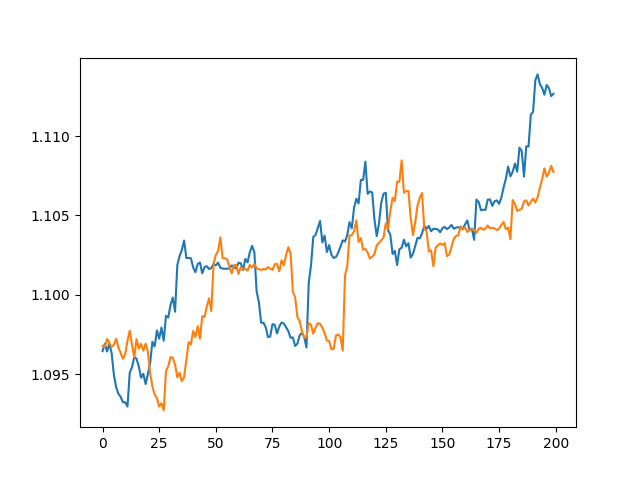
\includegraphics[width=0.9\textwidth]{240.png}
        \caption{4 hour predictions}
        \label{fig:240}
    \end{figure}

    \begin{figure}[htbp]
        \centering
        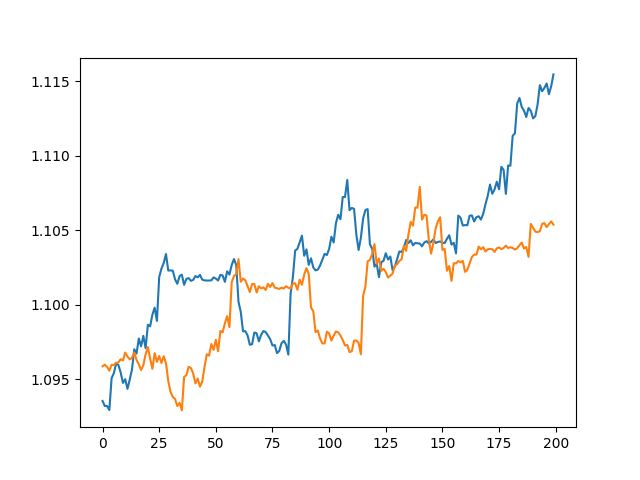
\includegraphics[width=0.9\textwidth]{480.png}
        \caption{8 hour predictions}
        \label{fig:480}
    \end{figure}


\pagebreak
\section{Source Code}
    \subsection{Networks}
        \subsubsection{Training}
        The test data used to train the networks could no longer be found on Kaggle. It has not been included below.    
        \vspace{5mm}\linebreak
            \textbf{lstmPrice.py}\vspace{3mm}
            \inputminted[linenos=true, xleftmargin=2pt, tabsize=4, breaklines]{python}{../source/nets/models/lstmPrice.py}
            \pagebreak
            \textbf{process.py}\vspace{3mm}
            \inputminted[linenos=true, xleftmargin=2pt, tabsize=4, breaklines]{python}{../source/nets/process.py}
            \pagebreak
            \textbf{train.py}\vspace{3mm}
            \inputminted[linenos=true, xleftmargin=2pt, tabsize=4, breaklines]{python}{../source/nets/train.py}
            \pagebreak
            \textbf{trainLSTM.py}\vspace{3mm}
            \inputminted[linenos=true, xleftmargin=2pt, tabsize=4, breaklines]{python}{../source/nets/trainLSTM.py}
            \pagebreak
            \textbf{assess.py}\vspace{3mm}
            \inputminted[linenos=true, xleftmargin=2pt, tabsize=4, breaklines]{python}{../source/nets/assess.py}

            \pagebreak
        \subsubsection{Testing Networks}
            The following source code was used as part of the testing \vspace{5mm}\linebreak
            \textbf{checkProcess.py}
            \inputminted[linenos=true, xleftmargin=2pt, tabsize=4, breaklines]{python}{../source/nets/checkProcess.py}
            \pagebreak
            This is an example of how the test data for the simple trends were created.\vspace{5mm}\linebreak
            \textbf{sineNoise.py}
            \inputminted[linenos=true, xleftmargin=2pt, tabsize=4, breaklines]{python}{../source/nets/sineNoise.py}
            \pagebreak
            \textbf{graphAll.py}
            \inputminted[linenos=true, xleftmargin=2pt, tabsize=4, breaklines]{python}{../source/nets/graphAll.py}

    \pagebreak
    \subsection{Site}
        \subsubsection{Back-End}
            \textbf{config.py}\vspace{3mm}
            \inputminted[linenos=true, xleftmargin=2pt, tabsize=4, breaklines]{python}{../source/site/config.py}
            \vspace{5mm}\textbf{database.py}\vspace{3mm}
            \inputminted[linenos=true, xleftmargin=2pt, tabsize=4, breaklines]{python}{../source/site/database.py}
            \vspace{5mm}\textbf{models.py}\vspace{3mm}
            \inputminted[linenos=true, xleftmargin=2pt, tabsize=4, breaklines]{python}{../source/site/models.py}
            \pagebreak
            \textbf{app.py}\vspace{3mm}
            \inputminted[linenos=true, xleftmargin=2pt, tabsize=4, breaklines]{python}{../source/site/app.py}
            \pagebreak
            \textbf{update.py}\vspace{3mm}
            \inputminted[linenos=true, xleftmargin=2pt, tabsize=4, breaklines]{python}{../source/site/update.py}
            \pagebreak
            \textbf{api.py}\vspace{3mm}
            \inputminted[linenos=true, xleftmargin=2pt, tabsize=4, breaklines]{python}{../source/site/api.py}
            \pagebreak
            \textbf{jsonPredictions.py}\vspace{3mm}
            \inputminted[linenos=true, xleftmargin=2pt, tabsize=4, breaklines]{python}{../source/site/jsonPredictions.py}

        \pagebreak
        \subsubsection{Front-End}
            \textbf{site.css}\vspace{3mm}
            \inputminted[linenos=true, xleftmargin=2pt, tabsize=4, breaklines]{css}{../source/site/static/site.css}
            \pagebreak
            \textbf{layout.html}\vspace{3mm}
            \inputminted[linenos=true, xleftmargin=2pt, tabsize=4, breaklines]{html}{../source/site/templates/layout.html}
            \pagebreak
            \textbf{home.html}\vspace{3mm}
            \inputminted[linenos=true, xleftmargin=2pt, tabsize=4, breaklines]{html}{../source/site/templates/home.html}
            \pagebreak
            \textbf{api.html}\vspace{3mm}
            \inputminted[linenos=true, xleftmargin=2pt, tabsize=4, breaklines]{html}{../source/site/templates/api.html}
            \pagebreak
            \textbf{showKey.html}\vspace{3mm}
            \inputminted[linenos=true, xleftmargin=2pt, tabsize=4, breaklines]{html}{../source/site/templates/showKey.html}
            \pagebreak
            \textbf{about.html}\vspace{3mm}
            \inputminted[linenos=true, xleftmargin=2pt, tabsize=4, breaklines]{html}{../source/site/templates/about.html}

